\section{Methods}\label{s:methods}

\subsection{Statistical Analysis Of Field Data}\label{s:methods_stats}

To frame the question of just how much variability in indoor air contaminant concentrations is actually observed, field datasets have been analyzed.
For this purpose, datasets from the ASU house in Utah, the EPA Indianapolis site and North Island NAS were chosen for analysis.
Readers are referred to the original published works for details regarding data acquisition\cite{holton_evaluation_2015,guo_vapor_2015,holton_temporal_2013,hosangadi_high-frequency_2017,u.s._environmental_protection_agency_assessment_2015}.\par

The ASU house data were obtained over a period of several years.
During part of this time, controlled pressure method (CPM) tests were being conducted, in which the house was underpressurized to an extent greater than that characterizing “normal” house operation: increasing VI potential\cite{mchugh_evaluation_2012,mchugh_recent_2017,holton_evaluation_2015}.
The period of CPM testing is thus excluded from the analysis.
Likewise, the existence of a preferential pathway at the ASU house needs to be considered in examining that dataset; during some of the testing at that site, this pathway was cut off, resulting in “normal” VI conditions in which the main source of contaminant was diffusion of contaminant vapor from an underlying groundwater source.\par

The NAS North Island dataset has not (as far as is known) been influenced by a preferential pathway, but the structure there was subject to “large” internal pressure fluctuations.
By “large” is meant still only of order 10-20 Pa, but these were greater than those generally recorded at the ASU house during normal operations.
The underlying soil at NAS North Island is sandy\cite{hosangadi_high-frequency_2017} and more permeable than that at the ASU site, which will be shown to lead to greater pressure sensitivity in the former case.\par

The Indianapolis site investigation also spanned a number of years and periodically included the testing of a sub-slab depressurziation system (SSD) for VI mitigation.
Only the period before the installation of this system was considered in the present analysis.
It is likely a sewer line beneath the structure acted as a preferential pathway\cite{mchugh_evidence_2017}.
Unlike at the ASU house, this preferential pathway was never removed or blocked, making it impossible to isolate the role of the preferential pathway at this site.
It is still of interest to consider the data from this site because of the completeness and extensiveness of the data collection.
Figure \ref{fig:indianapolis} illustrates a typical reported series of indoor air trichloroethylene (TCE) concentration measurements from this site.
There is almost a two order of magnitude variation in the concentration data.\par

\begin{figure}[htb!]
  \centering
 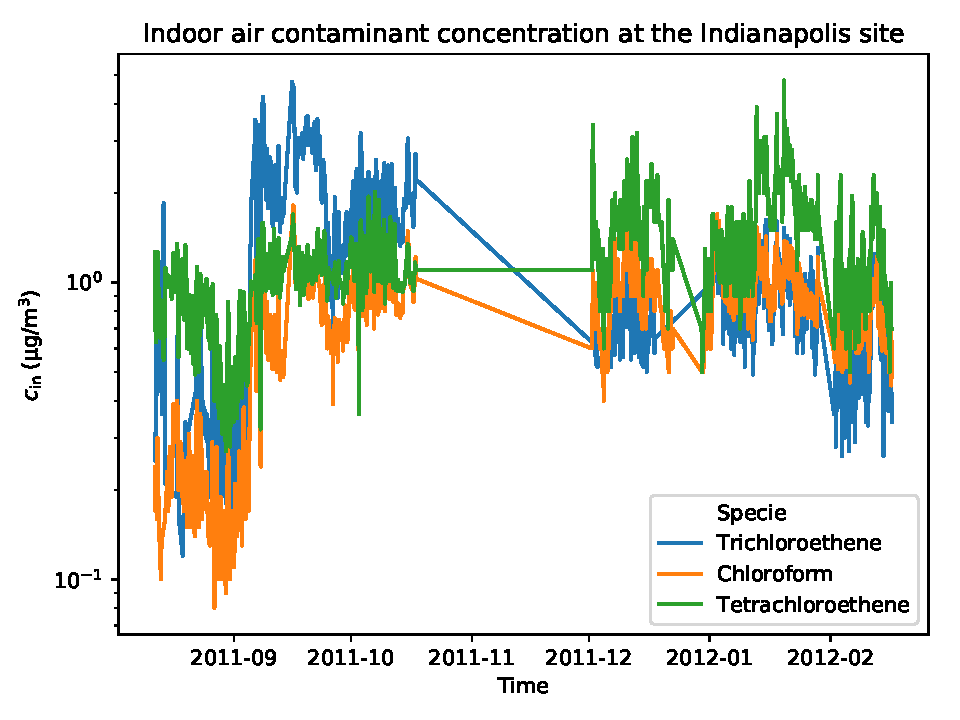
\includegraphics[width=\textwidth]{time_indianapolis.pdf}
 \caption{Typical data on indoor air TCE contaminant concentrations at the Indianapolis site\cite{u.s._environmental_protection_agency_assessment_2015}.}\label{fig:indianapolis}
\end{figure}

Some of the analysis of the above three field data sets relies on a probability density estimation technique called ”kernel density estimation” (KDE).
KDE is a technique used for estimating the probability distribution of a random variable(s) by using multiple kernels, or weighting functions to characterize the data sets.
In this case, Gaussian kernels are used to create the KDEs.
This means that it is presumed that the variables of interest (i.e., indoor air contaminant concentrations and indoor-outdoor pressure differentials, as sampled) are normally distributed around mean values and that there are statistical fluctuations associated with each sampling event.
In this instance, the scipy statistical package was used to construct the KDEs, assuming a bandwidth parameter determined by Scott’s rue.
The SciPy Python library was used to conduct all statistical analysis and data processing\cite{jones_scipy_2011}.\par

\subsection{Modeling Work}\label{s:methods_model}

A previously described three-dimensional computational fluid dynamics model of a generic VI impacted house has been used to elucidate certain aspects of transient VI processes.
In the present work, there has been an addition of a preferential pathway to the “standard” model that has been described before in publications by this group\cite{shen_influence_2013,yao_investigating_2017,yao_three-dimensional_2017}.
As in the earlier studies, only the vadose zone soil domain is directly modeled.
Figure \ref{fig:model} shows a cutaway view of the relevant modeling domain.\par

\begin{figure}[htb!]
  \centering
 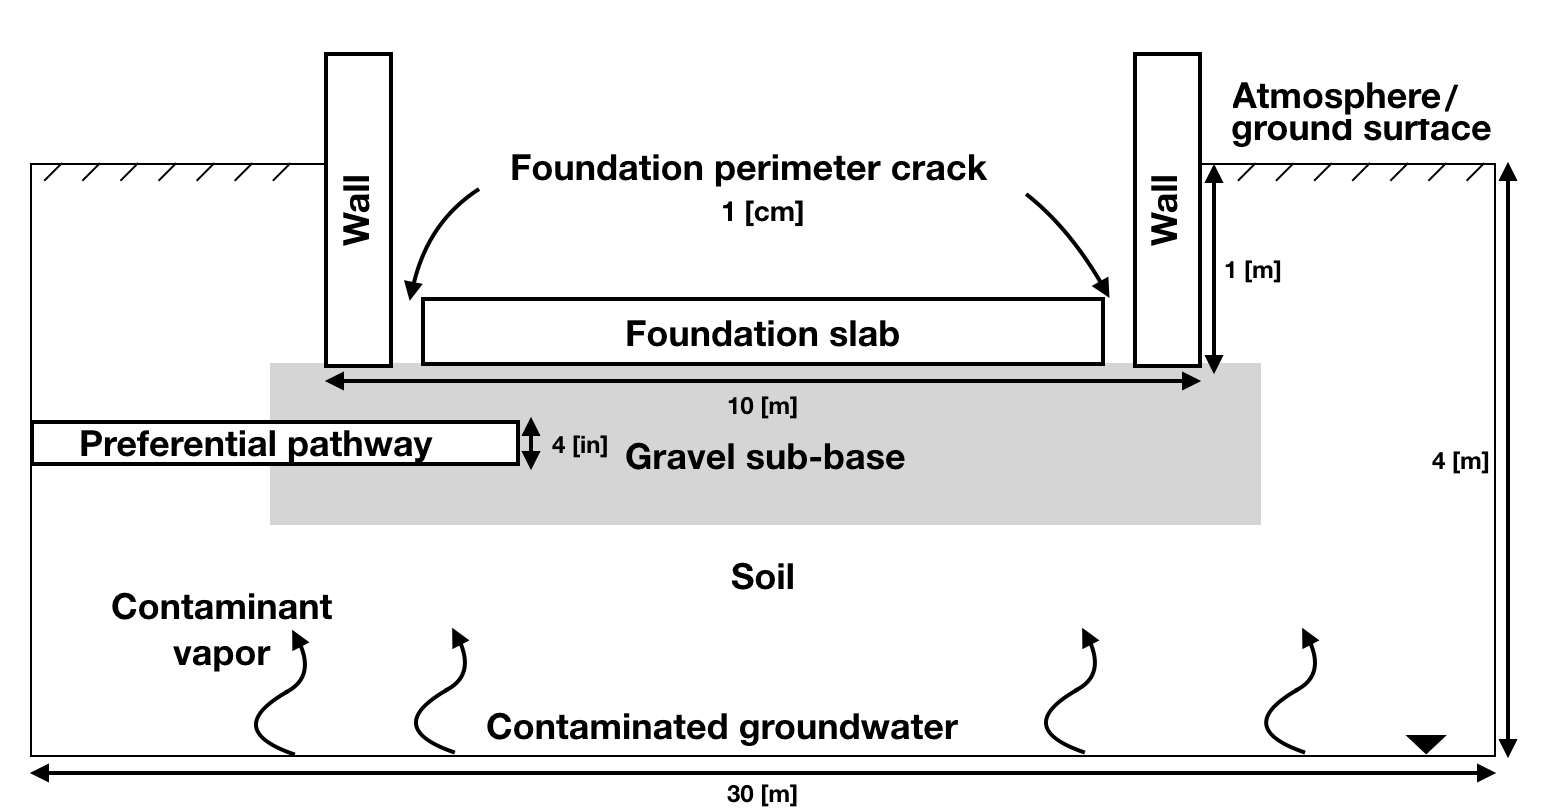
\includegraphics[width=\textwidth]{model.png}
 \caption{Foundation and vadose zone soil represented in the modeling. Note that here a gravel sub-base material is shown, but in certain simulations, that material is absent and the surrounding soil directly contacts the foundation slab.  Different assumptions are made regarding the preferential pathway, here shown as a pipe entering the gravel sub-base. In some cases, the preferential pathway has been "turned off".}\label{fig:model}
\end{figure}

The modeled VI impacted structure is assumed to have a 10x10 m foundation footprint, with the bottom of the foundation slab lying 1 m below ground surface (bgs), simulating a house with a basement.
The indoor air space is modeled as a continuously stirred tank (CST)\cite{u.s._environmental_protection_agency_oswer_2015} and all of the contaminant entering the house is assumed to enter with soil gas through a 1 cm wide crack located between the foundation walls and the foundation slab around the  perimeter of the house.
All of the contaminant leaving the indoor air space is assumed to do so via air exchange with the ambient.
The indoor control volume is here assumed to consist of only of the basement, having a total volume of $300 \; \mathrm{m^3}$.
Clearly different assumptions could be made regarding the structural features and the size of the crack entry route, but for present purposes, this is unimportant as the intent is only to show for “typical” values what the influence of some critical parameters is.\par

The modeled surrounding soil domain extends 5 meters from the perimeter of the house and is assumed to consist of sandy loam, except as noted otherwise.
Directly beneath the foundation slab, there is assumed to be a 30 cm (one foot) thick gravel layer, except in certain cases here this sub-base material is assumed to be the same as the surrounding soil (termed a "uniform" soil scenario).
The groundwater beneath the structure is assumed to be homogeneously contaminated with TCE selected as a prototypical contaminant.
The groundwater itself is not modeled, as the bottom of the model domain is defined by the top of the water table.
Where relevant, the preferential pathway is modeled as a 10 cm (4”) pipe that opens into the gravel sub-base beneath the structure.
The air in the pipe is also assumed to be contaminated with TCE at a vapor concentration equal to the vapor in equilibrium with the groundwater contaminant concentration below the structure, modified by a scaling factor $\chi$ (allowing the contaminant concentration in the pipe to be parameterized).
This model illustrates the concept of a "preferential pathway", as the pipe carries contaminant vapor to the immediate vicinity of the foundation, by a path that circumvents the usual soil diffusion pathway.\par

The ground surface and the pipe are both sources of air to the soil domain.
Both are assumed to exist at reference atmospheric pressure.
Soil gas transport is governed by Richard’s equation, a modified version of Darcy’s Law, taking the variability of soil moisture in the vadose zone into account\cite{richards_capillary_1931}.
The van Genuchten equations are used to predict the soil moisture content and thus the effective permeability of the soil\cite{van_genuchten_closed-form_1980}.
The effective diffusivity of contaminant in soil is calculated using the Millington-Quirk model\cite{millington_permeability_1961}.
The transport of contaminant vapor in the soil is assumed to be governed by the advection-diffusion equation, in which either advection or diffusion may dominate depending upon position and particular circumstances.
The key working equations and the boundary conditions are summarized in Table \ref{tbl:eqns_bc_parameters}.\par

\begin{table}[htb!]
  \setlength{\tabcolsep}{1pt}
  \centering
  \begin{tabular}{l c c c c c c}
    %%%%%%%%%%%%%%%%%%%%%%%%%%%%%%%%%%%%%%%%%%%%%%%%%%%%%%%%%%%%%%%%%%%%%%%%%%%%
    % GOVERNING EQUATIONS
    %%%%%%%%%%%%%%%%%%%%%%%%%%%%%%%%%%%%%%%%%%%%%%%%%%%%%%%%%%%%%%%%%%%%%%%%%%%%
    \toprule
    \multicolumn{7}{c}{\textbf{Governing Equations}} \\
    \midrule
    % CSTR
    Unsteady-CST & \multicolumn{6}{c}{$V\frac{d c_\mathrm{in}}{d t} = \int_{A_\mathrm{ck}} j_\mathrm{ck} dA - c_\mathrm{in} A_e V_\mathrm{slab}$} \\
    % RICHARDS
    Richard's & \multicolumn{6}{c}{$\nabla \cdot \rho \Big( - \frac{\kappa_s}{\mu} k_r \nabla p \Big) = 0$} \\
    % TRANSPORT
    Transport & \multicolumn{6}{c}{$\frac{\partial}{\partial t} \Big( \theta_w c_w + \theta_g c \Big) = \nabla (D_\mathrm{eff} \cdot \nabla c) - \vec{u} \cdot \nabla c$} \\
    % MILLINGTON-QUIRK
    Millington-Quirk & \multicolumn{6}{c}{$D_\mathrm{eff} = D_\mathrm{air}\frac{\theta_g^{10/3}}{\theta_t^2} + \frac{D_\mathrm{water}}{K_H} \frac{\theta_w^{10/3}}{\theta_t^2}$} \\
    % VAN GENUCHTEN
    \multirow{4}{*}{van Genuchten} & \multicolumn{6}{c}{$\mathrm{Se} = \frac{\theta_w - \theta_r}{\theta_t - \theta_r} = [1 + |\alpha z|^n]^{-m}$} \\
     & \multicolumn{6}{c}{$\theta_g = \theta_t - \theta_w$}\\
     & \multicolumn{6}{c}{$k_r = (1-\mathrm{Se})^{l}[1(\mathrm{Se}^{m})^m]^2$} \\
     & \multicolumn{6}{c}{$m = 1 - 1/n$} \\
     %%%%%%%%%%%%%%%%%%%%%%%%%%%%%%%%%%%%%%%%%%%%%%%%%%%%%%%%%%%%%%%%%%%%%%%%%%%%
     % BOUNDARY CONDITIONS
     %%%%%%%%%%%%%%%%%%%%%%%%%%%%%%%%%%%%%%%%%%%%%%%%%%%%%%%%%%%%%%%%%%%%%%%%%%%%
    \midrule
    \multicolumn{7}{c}{\textbf{Boundary Conditions}} \\
    \midrule
    \textbf{Boundary} & \multicolumn{3}{c}{\textbf{Richard's Eqn.}} & \multicolumn{3}{c}{\textbf{Transport Eqn.}} \\
    % Foundation crack
    Foundation crack & \multicolumn{3}{c}{$p = p_\mathrm{in/out} \; \mathrm{(Pa)}$} & \multicolumn{3}{c}{$j_\mathrm{ck} = \frac{u c}{1 - \exp{(u L_\mathrm{slab}/D_\mathrm{air})}}$} \\
    % Groundwater source
    Groundwater & \multicolumn{3}{c}{\textit{No flow}} & \multicolumn{3}{c}{$c = c_\mathrm{gw} K_H \; \mathrm{(\mu g/m^3)}$} \\
    % Ground surface
    Ground surface & \multicolumn{3}{c}{$p = 0 \; \mathrm{(Pa)}$} & \multicolumn{3}{c}{$c = 0 \; \mathrm{(\mu g/m^3)}$} \\
    % Preferential pathway
    \multirow{2}{*}{\begin{minipage}{0.2\textwidth}Preferential\\pathway\end{minipage}} & \multicolumn{3}{c}{\multirow{2}{*}{$p = 0 \; \mathrm{(Pa)}$}} & \multicolumn{3}{c}{\multirow{2}{*}{$c = c_\mathrm{gw} K_H \chi \; \mathrm{(\mu g/m^3)}$}} \\ \\
    %%%%%%%%%%%%%%%%%%%%%%%%%%%%%%%%%%%%%%%%%%%%%%%%%%%%%%%%%%%%%%%%%%%%%%%%%%%%
    % SOIL PROPERTIES
    %%%%%%%%%%%%%%%%%%%%%%%%%%%%%%%%%%%%%%%%%%%%%%%%%%%%%%%%%%%%%%%%%%%%%%%%%%%%
    \midrule
    \multicolumn{7}{c}{\textbf{Soil Properties}\cite{dan_capillary_2012,abreu_conceptual_2012,u.s._environmental_protection_agency_userss_2004}} \\
    \midrule
    \textbf{Soil} & \textbf{$\kappa_s \; \mathrm{(m^2)}$} & \textbf{$\theta_s$} & \textbf{$\theta_r$} & \textbf{$\alpha \; \mathrm{(1/m)}$} & \textbf{$n$} \\
    % GRAVEL
    Gravel & $1.3 \cdot 10^{-9}$ & 0.42 & 0.005 & 100 & 3.1 \\
    % SANDY LOAM
    Sandy Loam & $5.9 \cdot 10^{-13}$ & 0.39 & 0.039 & 2.7 & 1.4 \\
    %%%%%%%%%%%%%%%%%%%%%%%%%%%%%%%%%%%%%%%%%%%%%%%%%%%%%%%%%%%%%%%%%%%%%%%%%%%%
    % TCE PROPERTIES
    %%%%%%%%%%%%%%%%%%%%%%%%%%%%%%%%%%%%%%%%%%%%%%%%%%%%%%%%%%%%%%%%%%%%%%%%%%%%
    \midrule
    \multicolumn{7}{c}{\textbf{Trichloroethylene (diluted in air) Properties}\cite{abreu_conceptual_2012,u.s._environmental_protection_agency_userss_2004}} \\
    \midrule
     & \multicolumn{1}{c}{\textbf{$D_\mathrm{air} \; \mathrm{(m^2/h)}$}} & \textbf{$D_\mathrm{water} \; \mathrm{(m^2/h)}$} & \textbf{$\rho \; \mathrm{(kg/m^3)}$} & \textbf{$\mu \; \mathrm{(Pa \cdot s)}$} & \textbf{$K_H$} \\
     & \multicolumn{1}{c}{$2.47 \cdot 10^{-2}$} & $3.67 \cdot 10^{-6}$ & 1.614 & $1.86 \cdot 10^{-5}$ & 0.403 \\
    %%%%%%%%%%%%%%%%%%%%%%%%%%%%%%%%%%%%%%%%%%%%%%%%%%%%%%%%%%%%%%%%%%%%%%%%%%%%
    % BUILDING PROPERTIES
    %%%%%%%%%%%%%%%%%%%%%%%%%%%%%%%%%%%%%%%%%%%%%%%%%%%%%%%%%%%%%%%%%%%%%%%%%%%%
    \midrule
    \multicolumn{7}{c}{\textbf{Building Properties}} \\
    \midrule
     & \multicolumn{1}{c}{\textbf{$V_\mathrm{base} \; \mathrm{(m^3)}$}} & \textbf{$L_\mathrm{slab} \; \mathrm{(cm)}$} & \textbf{$A_e \; \mathrm{(1/hr)}$} \\
     & \multicolumn{1}{c}{300} & 15 & 0.5 \\
    \bottomrule
  \end{tabular}
  \caption{Governing equations, boundary conditions \& model input parameters. See Table \ref{tbl:abbreviations} for nomenclature.}\label{tbl:eqns_bc_parameters}
\end{table}
